\documentclass[a5paper,DIV=12,BCOR=9mm,headsepline,headings=small,cleardoubleempty,10pt]{scrbook}
\usepackage{scrpage2}
\usepackage{Open-Advice 2}
\usepackage[utf8]{inputenc}
\usepackage{textcomp}
\usepackage{graphicx}
\usepackage{xcolor}
\usepackage{tabularx}
\usepackage[english]{babel}
\usepackage[raiselinks=true,
bookmarks=true,
bookmarksopenlevel=1,
bookmarksopen=true,
bookmarksnumbered=true,
hyperindex=true,
plainpages=false,
pdfpagelabels=true,
pdfborder={0 0 0.5}
]{hyperref}
\usepackage[textsize=tiny]{todonotes}

% Meta data
\newcommand{\booktitle}{Open Advice 2}
\newcommand{\booksubtitle}{ADD SUBTITLE}
\newcommand{\bookeditor}{Lydia Pintscher}
\newcommand{\bookyear}{2013}
\newcommand{\bookisbn}{ADD ISBN}
\newcommand{\bookurl}{http://open-advice.org}
\newcommand{\bookauthors}{ADD AUTHORS}

\hypersetup{
  pdfauthor={\bookauthors},
  pdftitle={\booktitle},
  pdfsubject={Open Source, Free Software},
  pdfkeywords={Open Source, Free Software},
  pdflang=en,
  colorlinks,
  linkcolor=black,
  anchorcolor=black,
  filecolor=black,
  urlcolor=black,
  citecolor=black,
  bookmarksnumbered=true,
  pdfpagelayout=TwoColumnRight
}
\ifusinght
\else
  \usepackage{xmpincl}
  \includexmp{Open-Advice}
  \usepackage{pdfpages}
\fi

\pagestyle{scrheadings}
\ihead[]{\headmark}
\ohead[]{\pagemark}
%\cfoot[]{Open Advise 2}
\ifoot[]{ }
\ofoot[]{ }

% Use a nicer-Looking design for the TOC
\usepackage{tocstyle}
\usetocstyle{KOMAlike}

% Avoid typographical unpleasantries
\clubpenalty = 10000
\widowpenalty = 10000
\displaywidowpenalty = 10000
% Avoids line-overshooting at the cost of "Word-like" spacing
\setlength{\emergencystretch}{0.25em}

\begin{document}
\ifusinght
\else
  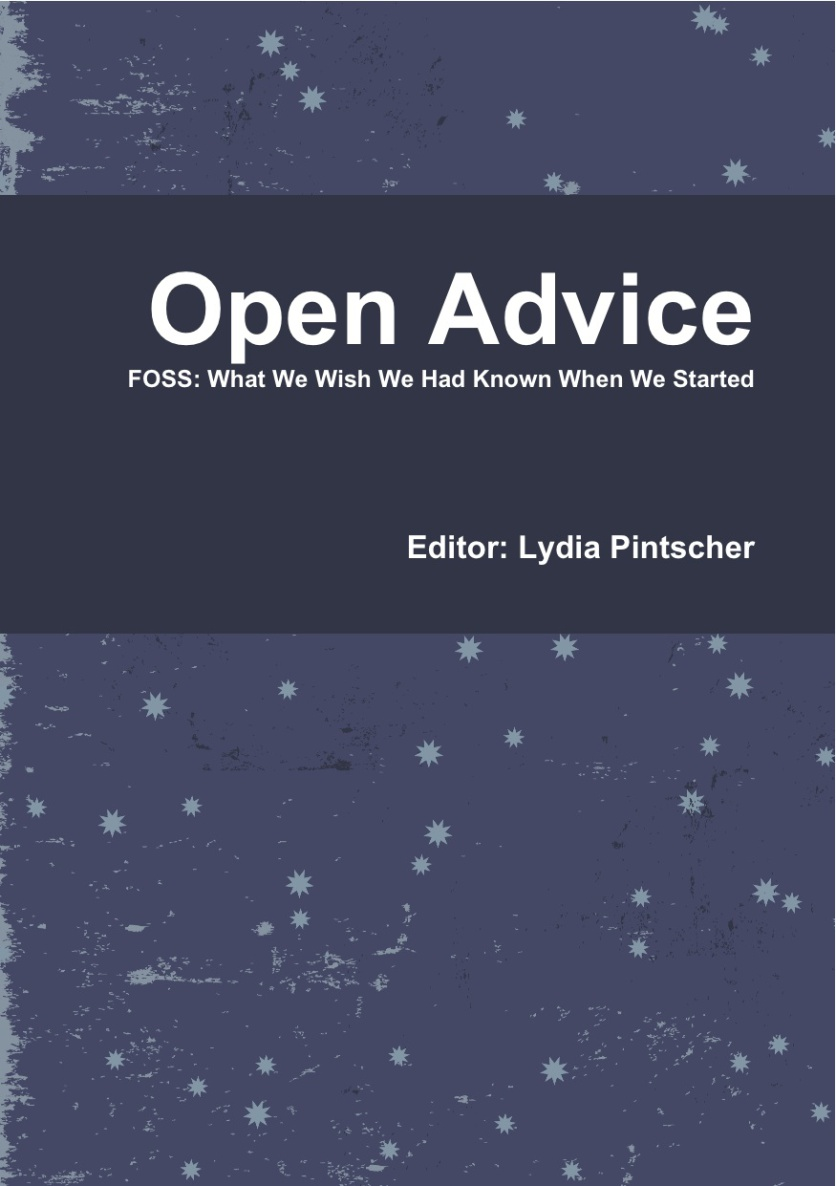
\includepdf[noautoscale]{frontcover}
\fi
\frontmatter
\thispagestyle{empty}
% Extra title page
\booktitle
\newpage
% empty page back
\newpage
% inner title page
\begin{titlepage}
\begin{flushright}
\bookeditor{} (Editor)\\
\vspace{10em}
{\Huge\bfseries\sffamily\booktitle}\\
\vspace{2em}
{\large\sffamily\booksubtitle}
\end{flushright}
\end{titlepage}
% titleback
\thispagestyle{empty}
The information in this book is distributed on an ``As Is'' basis, without warranty. While every precaution has been taken in the preparation of this work, neither the authors nor the editor or publishers shall have any liability to any person or entity with respect to any loss or damage caused or alledged to be caused directly or indirectly by the information contained in it.%
\vfill
Copyright \textcopyright{} \bookyear{} \bookauthors\\
\newline
\fbox{\parbox{\textwidth}{
\begin{center}
\includegraphics{cc-by-sa.png}\end{center}
This work is licensed under a Creative Commons Attribution-ShareAlike 3.0 License. To view a copy of this license visit: \\{\small\url{http://creativecommons.org/licenses/by-sa/3.0/legalcode}}.
\vspace{0.25em}
}}
\newline \\
Visit \url{http://www.open-advice.org} to download this book as PDF or eBook and receive additional information.
\newline \\
{\tt ISBN: \bookisbn}%
%dedication
\newpage
\thispagestyle{empty}
\vspace*{2cm}
\begin{flushright}
{\Large\itshape TO BE WRITTEN}\\
\end{flushright}
\newpage
\thispagestyle{empty}
\mbox{}
\newpage
%End of top matter

\section*{Foreword}

\todo{add ISBN}
\todo{add authors}
\todo{add dedication}
\todo{add subtitle}
\todo{add backmatter text}
\todo{replace cover image}
\todo{find author for foreword}
\todo[inline]{write foreword}

\newpage

\section*{Thank You!}

This book would not have been possible without the support of each of the
authors and the following people, who helped make it happen:
\begin{itemize}
 \item ADD! \todo{add people}
\end{itemize}

\newpage

\tableofcontents
\listoftodos
\mainmatter
%\input{foo}
\chapter*{Closing}

\todo[inline]{write closing words}

\backmatter
\end{document}
